\subsection{Support Vector Machines}
\label{sec:svmExperiments-ta}
	Firstly, we investigate the case when no kernels are used. Then we will investigate the use of two possible kernels -- polynomial (degree 3) and radial basis function. We will train on the first ten records using the \verb!MATLAB!\textsuperscript{\textregistered}'s function \verb!svmtrain!. Then we will test our trained parameters on the next five records, where we record the accuracy as the ratio of the number of correctly classified annotations over the total number of annotations. We will also record the number of Support Vectors (SVs) because they indicate the generalisation performance. The actual implementation can be found in Appendix \ref{ch:SVMCode}.

\subsubsection{No kernels}
	The results of this experiment are shown in Figure \ref{fig:svmExperimentNoKernels} and in Table \ref{table:svmResults}. The accuracy is high, however so is the number of SV's. This indicates that the generalisation guarantee is poor.
	\begin{figure}[ht]
		\centering
		\subfloat[record 11]{%
			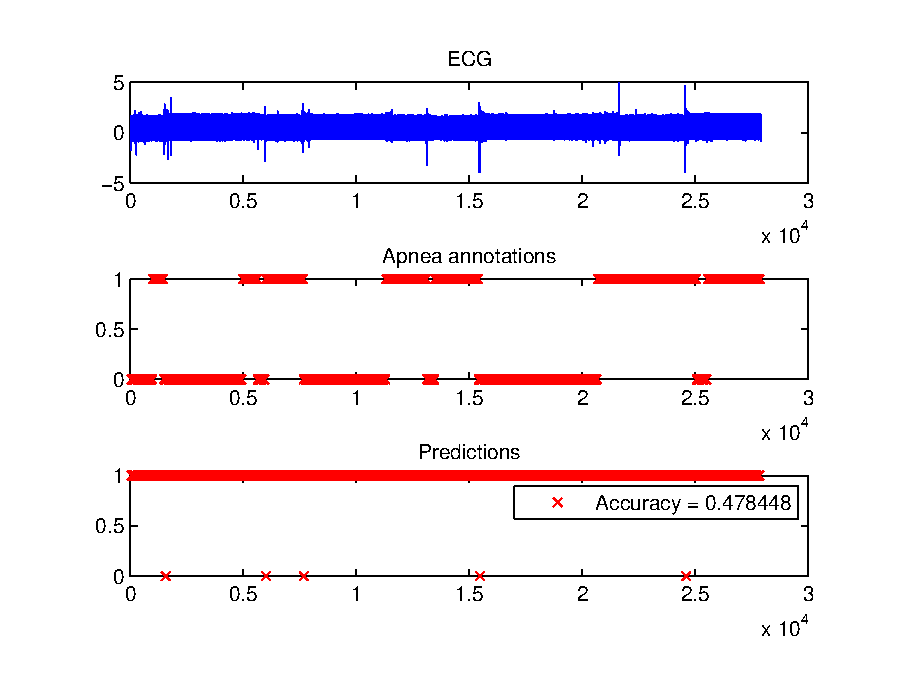
\includegraphics[width=.33\textwidth]{drawings/svm/svmTestNoKernel11}}
		\subfloat[record 12]{%
			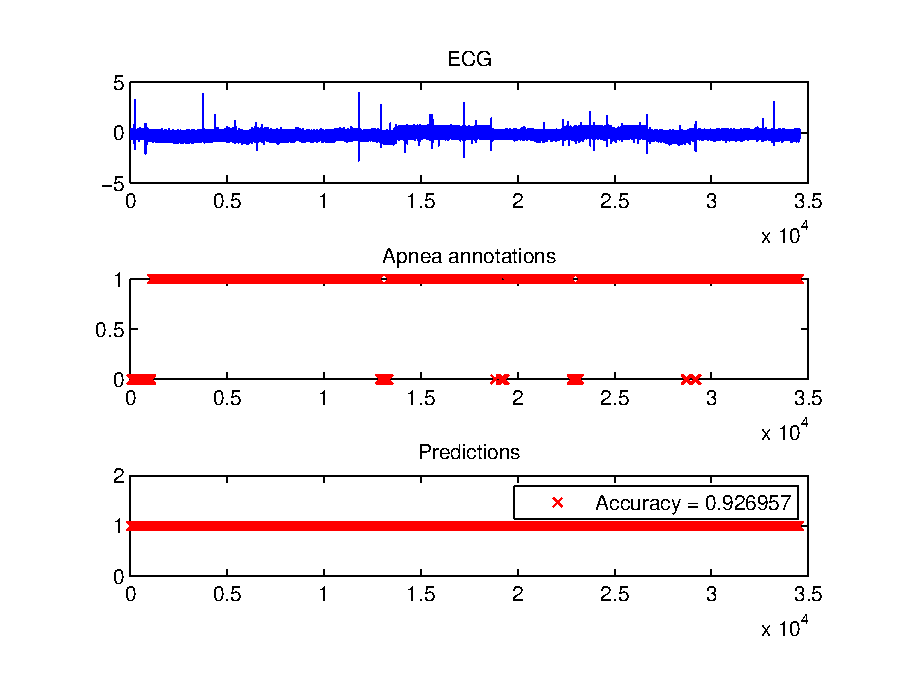
\includegraphics[width=.33\textwidth]{drawings/svm/svmTestNoKernel12}}
		\subfloat[record 13]{%
			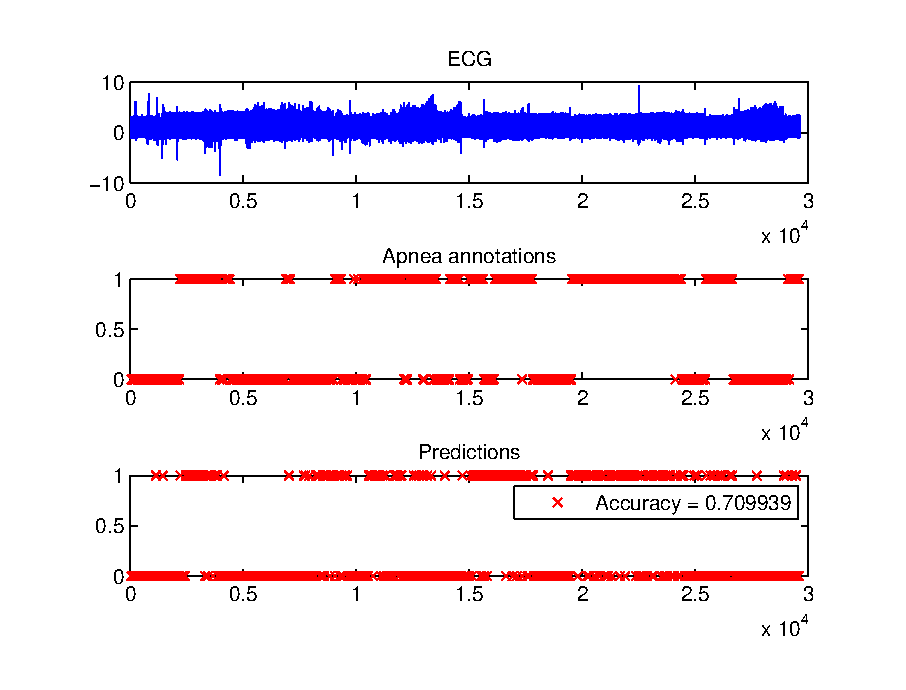
\includegraphics[width=.33\textwidth]{drawings/svm/svmTestNoKernel13}} \\
		\subfloat[record 14]{%
			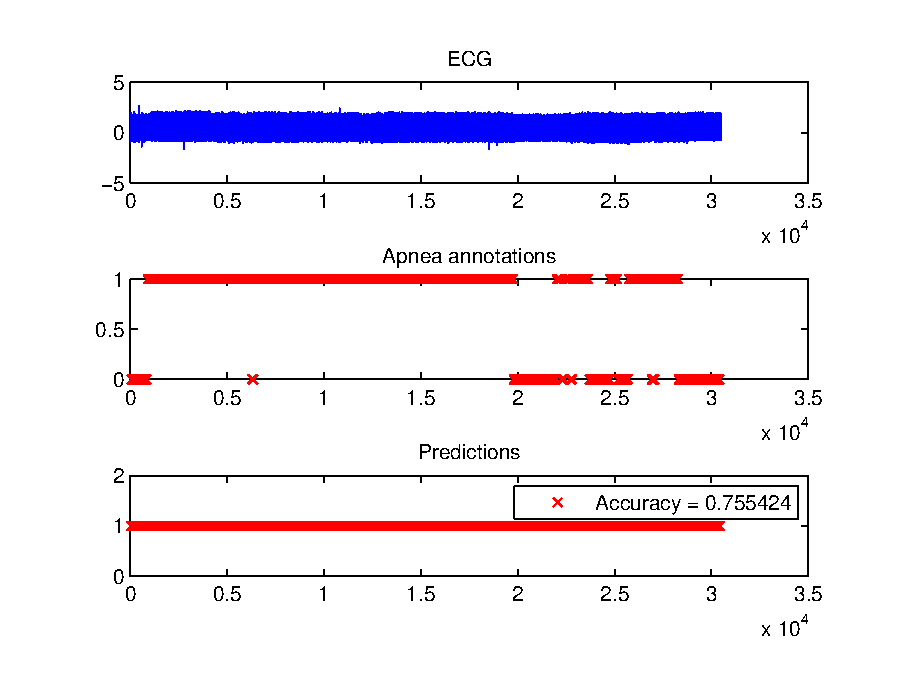
\includegraphics[width=.33\textwidth]{drawings/svm/svmTestNoKernel14}}
		\subfloat[record 15]{%
			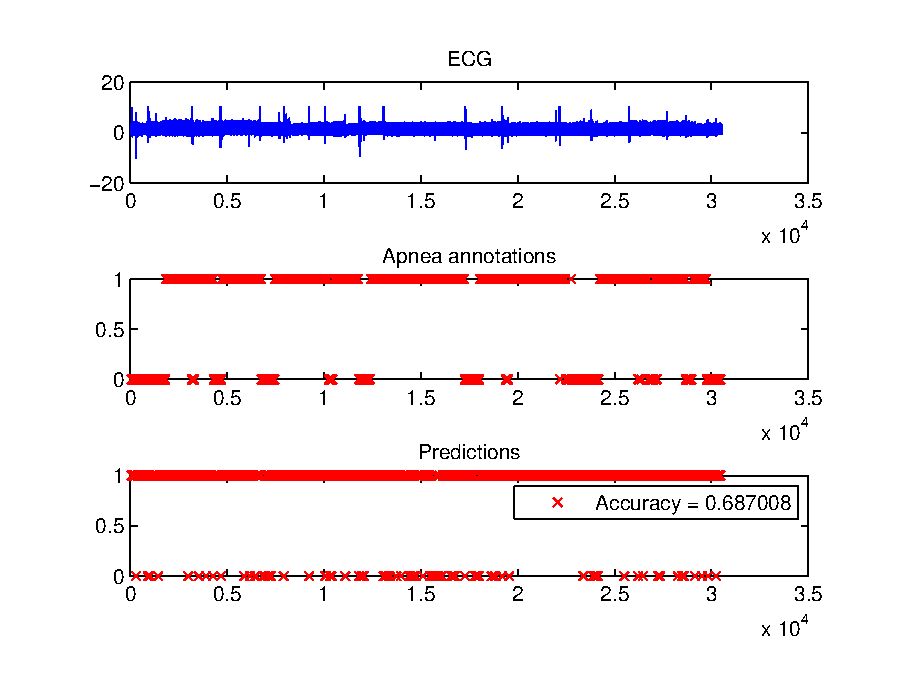
\includegraphics[width=.33\textwidth]{drawings/svm/svmTestNoKernel15}}
		\caption{Performance of no kernels on the test records 11 to 15}
		\label{fig:svmExperimentNoKernels}
	\end{figure}

\subsubsection{Polynomial kernel}
	The results of this experiment are shown in Figure \ref{fig:svmExperimentPoly} and in Table \ref{table:svmResults}. We can see that there is a low number of SVs and high accuracy. This means that the polynomial kernel is likely to perform well on unseen data. If we had more computational resources, we could have used more features (and correspondingly more training data) in order to represent the features better.
	\begin{figure}[ht]
		\centering
		\subfloat[record 11]{%
			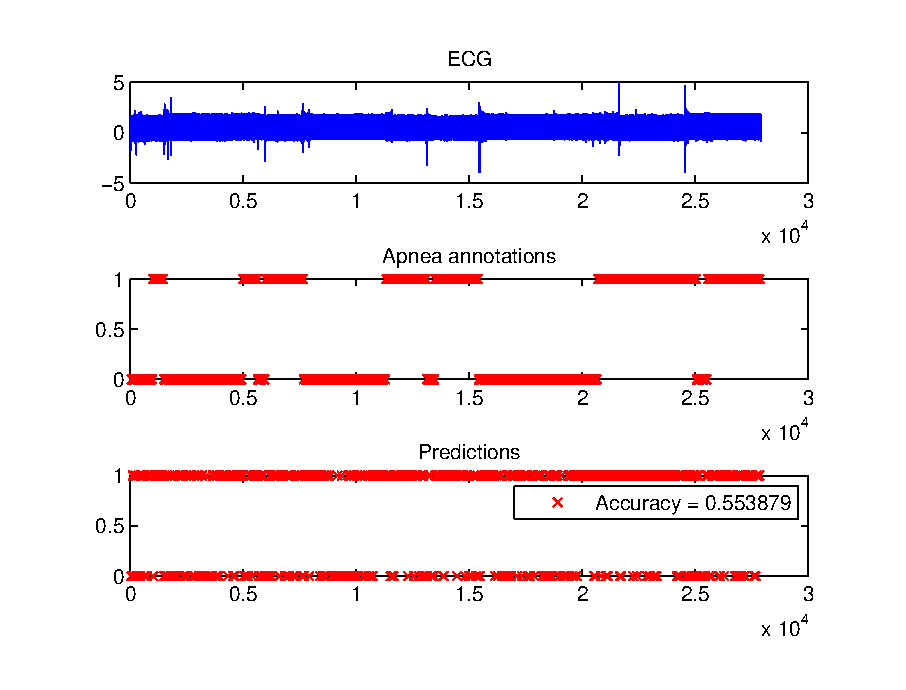
\includegraphics[width=.33\textwidth]{drawings/svm/svmTestPoly11}}
		\subfloat[record 12]{%
			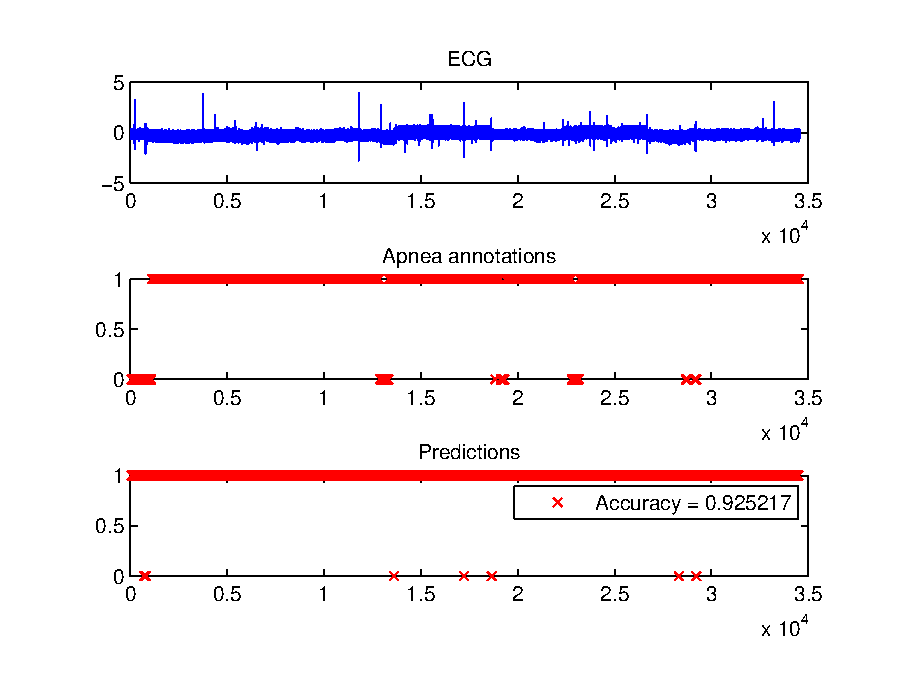
\includegraphics[width=.33\textwidth]{drawings/svm/svmTestPoly12}}
		\subfloat[record 13]{%
			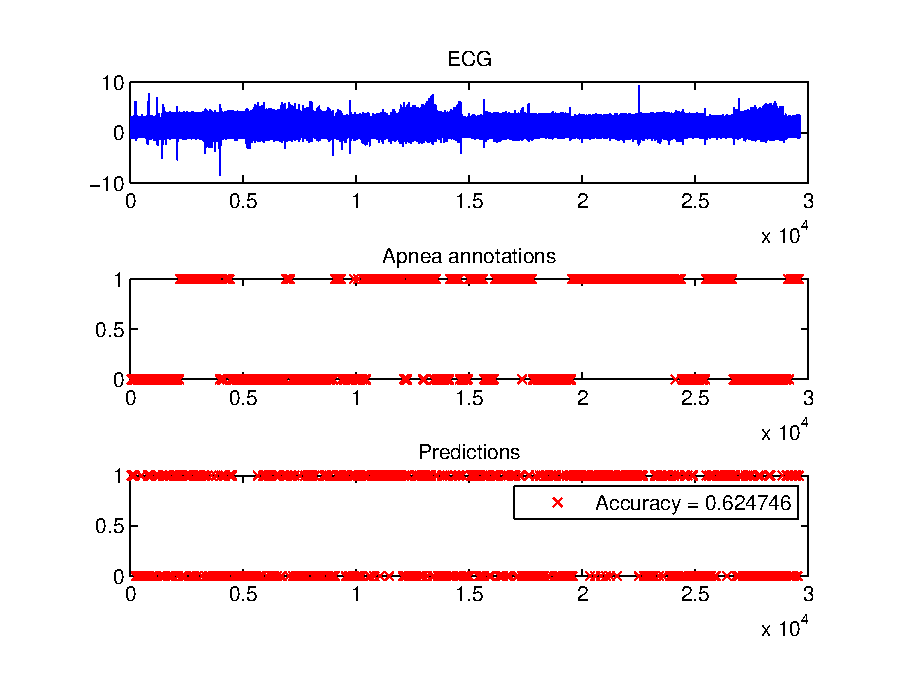
\includegraphics[width=.33\textwidth]{drawings/svm/svmTestPoly13}} \\
		\subfloat[record 14]{%
			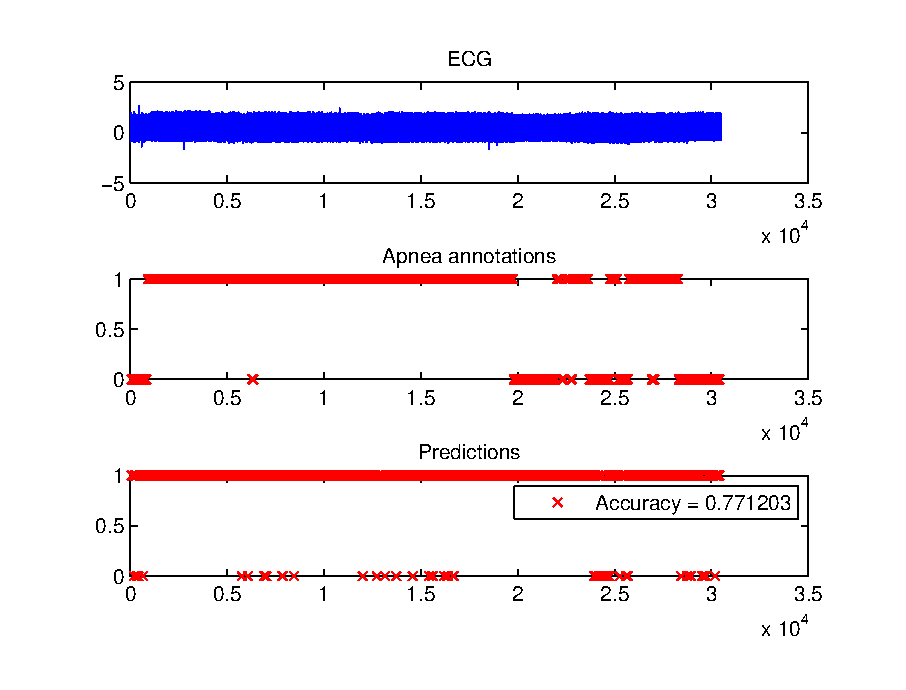
\includegraphics[width=.33\textwidth]{drawings/svm/svmTestPoly14}}
		\subfloat[record 15]{%
			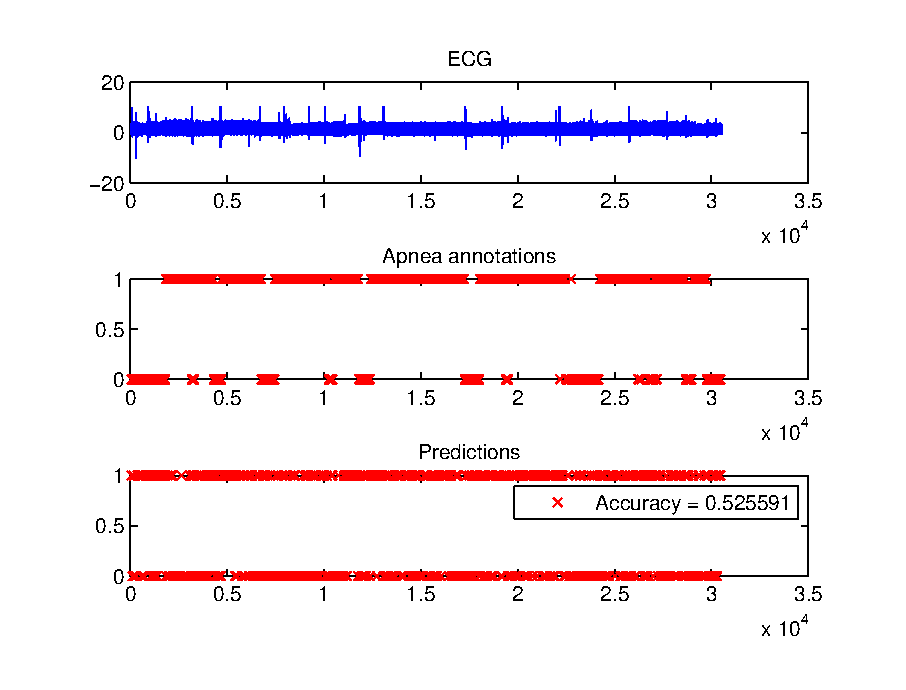
\includegraphics[width=.33\textwidth]{drawings/svm/svmTestPoly15}}
		\caption{Performance of the polynomial kernel on the test records 11 to 15}
		\label{fig:svmExperimentPoly}
	\end{figure}

\subsubsection{Radial basis function kernel}
	The results of this experiment are shown in Figure \ref{fig:svmExperimentRbf} and in Table \ref{table:svmResults}. Similarly to the case of no kernels, the accuracy is high, but so is the number of SV's indicating poor generalisation performance.
	\begin{figure}[ht]
		\centering
		\subfloat[record 11]{%
			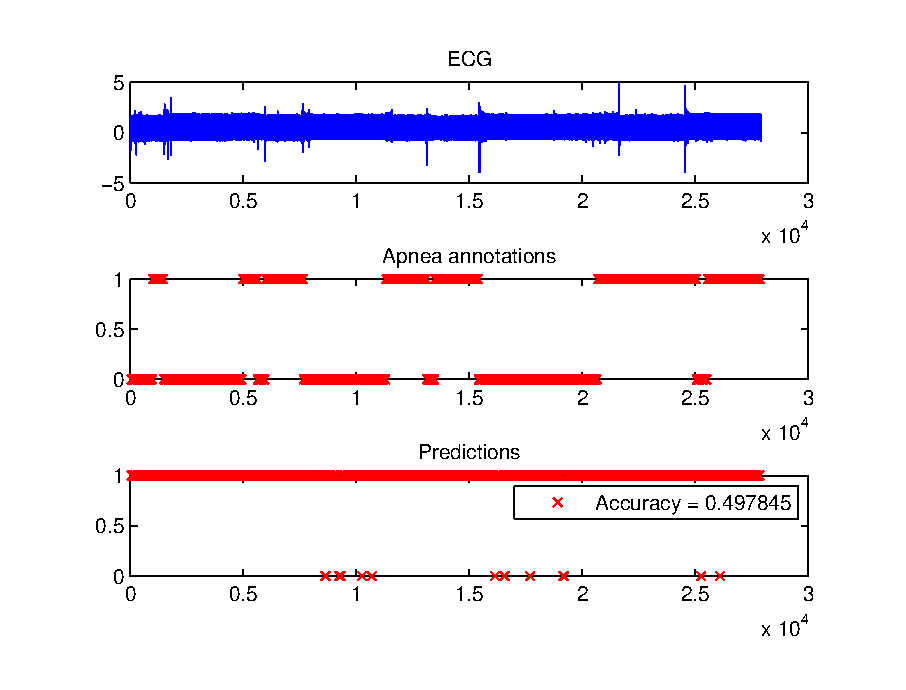
\includegraphics[width=.33\textwidth]{drawings/svm/svmTestRbf11}}
		\subfloat[record 12]{%
			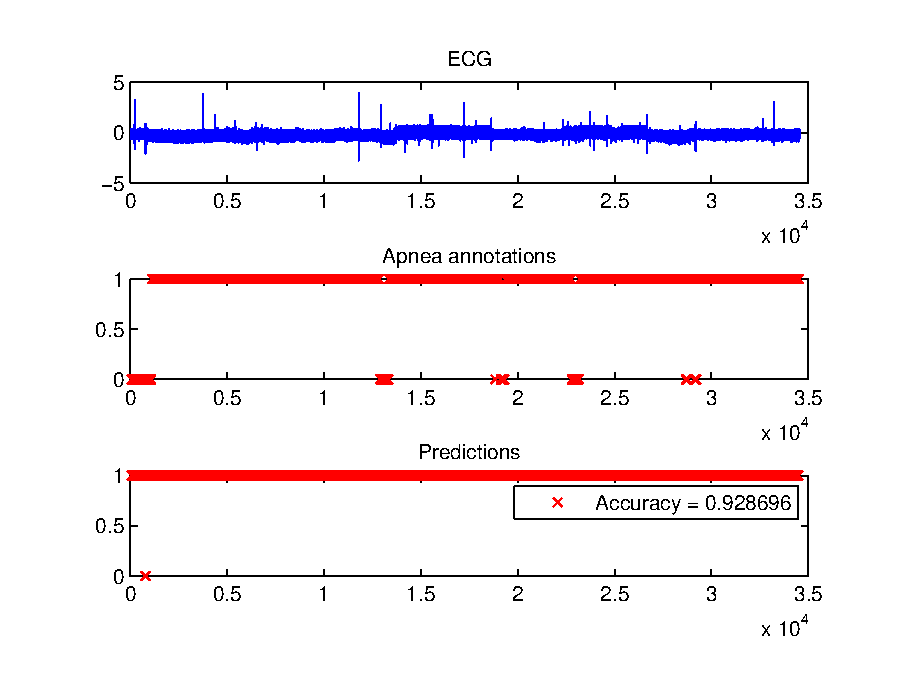
\includegraphics[width=.33\textwidth]{drawings/svm/svmTestRbf12}}
		\subfloat[record 13]{%
			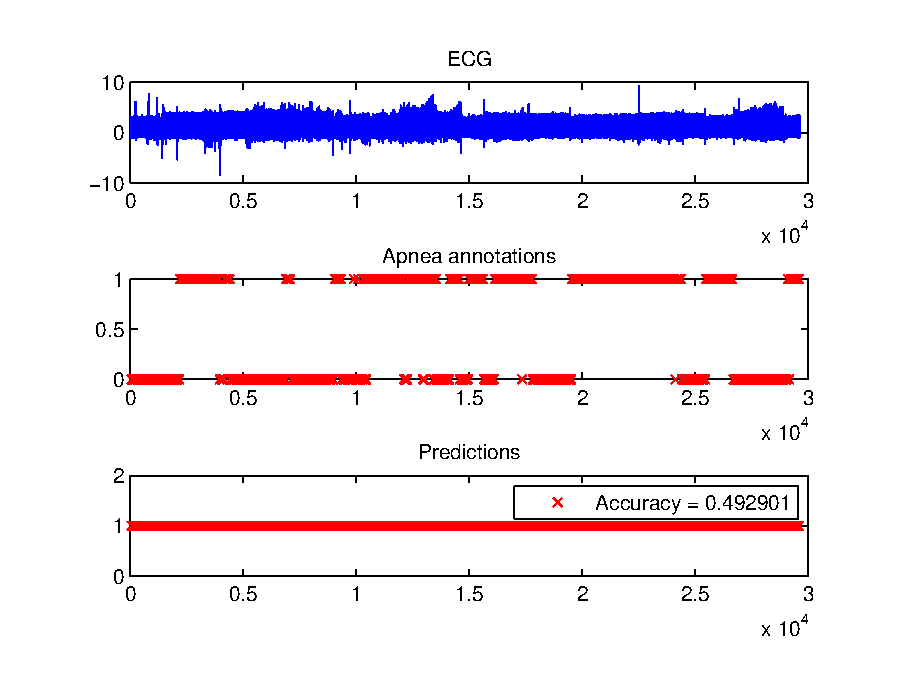
\includegraphics[width=.33\textwidth]{drawings/svm/svmTestRbf13}} \\
		\subfloat[record 14]{%
			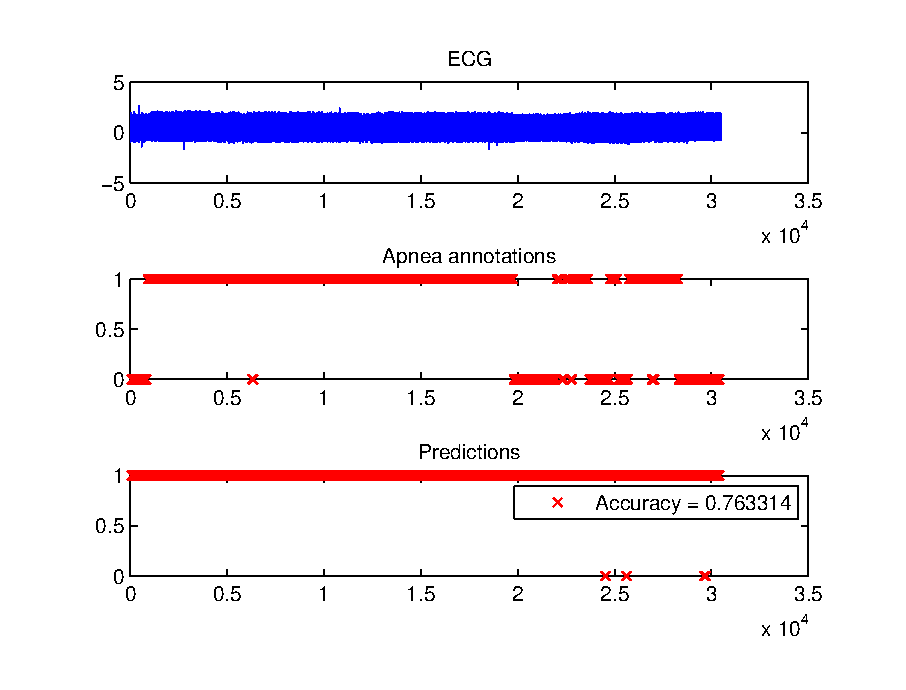
\includegraphics[width=.33\textwidth]{drawings/svm/svmTestRbf14}}
		\subfloat[record 15]{%
			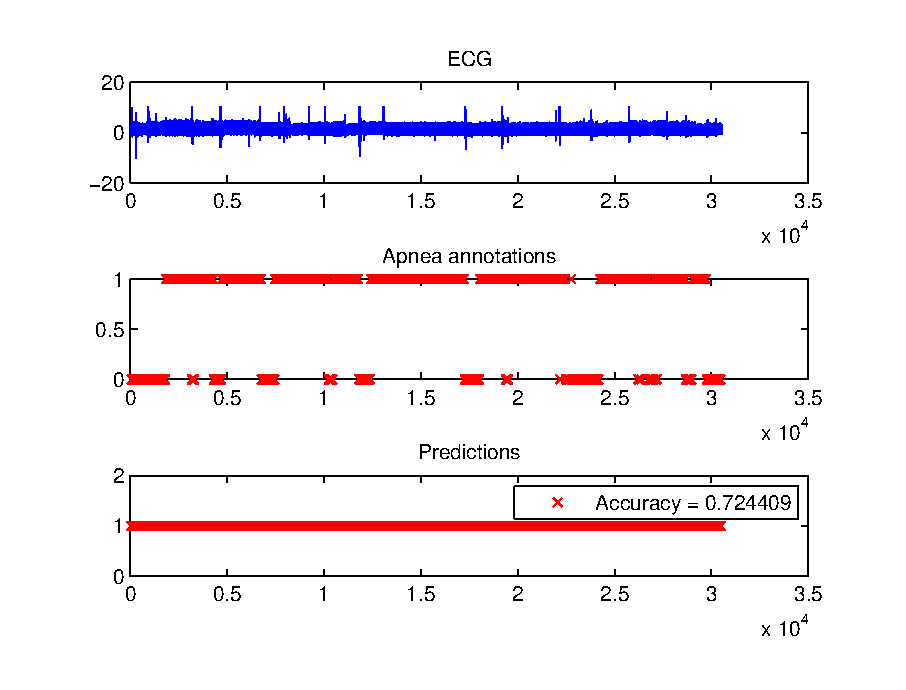
\includegraphics[width=.33\textwidth]{drawings/svm/svmTestRbf15}}
		\caption{Performance of the Radial Basis Function kernel on the test records 11 to 15}
		\label{fig:svmExperimentRbf}
	\end{figure}

\subsubsection{Summary}
	Summary of the performances of the different kernels is shown in Table \ref{table:svmResults}. The polynomial kernel with degree 3 is the most promising in terms of generalisation. All three kernels have similar accuracy. If we had more computational resources, we could have done deeper analysis and tests, e.g. use more principal components to capture as much variance as possible and use more training data (we only used 10 out of 35).
	\begin{table}[h]
		\centering
		\begin{tabular}{@{}lll@{}}
		\toprule
		            & \# SV's (5005 data points) & Average accuracy \\ \midrule
		No kernel   & 3679                       & 0.7116           \\
		Poly kernel & 1879                       & 0.6801           \\
		Rbf kernel  & 4033                       & 0.6814           \\ \bottomrule
		\end{tabular}
		\caption{Summary of performances of different kernels}
		\label{table:svmResults}
	\end{table}